
\subsection{Literature Overview}
The study of ladder lottieres as mathematical objects began in 2010, in  the paper
\textbf{Efficient Enumeration of Ladder Lotteries and its Application}. The paper was 
written by four authors, Yamanaka, Horiyama, Uno and Wasa. In this paper the 
authors present an algorithm for generating all the ladder lotteries of an 
arbitrary permutation, $\pi$. Since this paper emerged, there have been 
several other paper written directly about ladder lotteries. 
These papers include \textbf{The Ladder Lottery Realization Problem},
\textbf{Optimal Reconfiguration of Optimal Ladder Lotteries}, 
\textbf{Efficient Enumeration of all Ladder Lotteries with K Bars},
\textbf{Coding Ladder Lotteries} and
\textbf{Enumeration, Counting, and Random Generation of Ladder Lotteries}.
\subsection{Efficient Enumeration of Laddder Lotteries and its Application}
In their paper, Efficient Enumeration of Ladder Lotteries and its Application,
the authors provide an algorithm for generating $OptL\{\pi\}$ 
for any $\pi$, in $\mathcal{O}(1)$ per ladder. This is the first and only 
published algroithm for generating $OptL\{\pi\}$. The paper also presents the number 
of ladder lotteries in $OptL\{(11, 10, 9, 8, 7, 6, 5, 4, 3, 2, 1)\}$ which is 
$5,449,192,389,984$. This is a very impressive accomplishment for reasons which 
will be discussed later in the literature review.\par 
The authors' algorithm is based on several key concepts, the most 
important of which is the \emph{local swap operation}. This is the 
minimal change operation that transitions from one ladder in $OptL\{\pi\}$ to the 
next ladder. The local swap operation is essentially a 180 degree rotation
of three bars in the ladder, all at different levels in the ladder, such that the bottom
bar is rotated to the top, the middle bar stays in the middle and the top bar
is rotated to the bottom. If the bars undergo a 180 degree rotation to the right, 
then this is known as a \emph{right swap operation} and 
if the bars udergo a 180 degree rotation to the left then this 
is known as a \emph{left swap operation}. To go to the next ladder in the set, 
the current ladder, $L_{i}$ udergoes a right swap operation 
to get toe ladder $L_{i+1}$. See figure --ref-- for an exmaple of a 
local swap operation. The \emph{route} of an element is the sequence of bars in the ladder, from top left to 
bottom right, that an element must cross in order to reach its correct position in 
the identity permutation. Note that each bar has two elements that cross it, 
therefore the bar belongs to the route of the greater of the two elements.
The \emph{clean level} refers to the smallest element 
in $\pi$ such that none of its bars have a bar of a lesser element above its route.
If there is no such element, then the clean level is the maximum element in $\pi$ + 1.

\begin{figure}[!htp]
	\label{fig:rightSwap}
	\begin{minipage}{0.4\textwidth}
		\begin{center}

			%%drawing the lines
			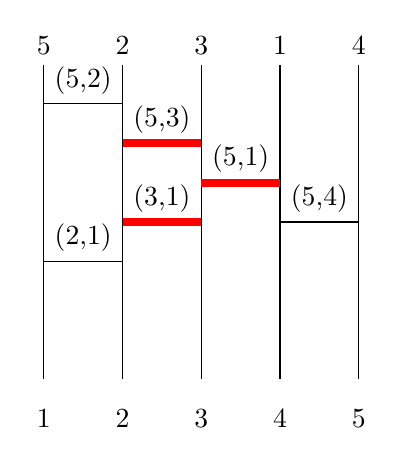
\begin{tikzpicture}
				\draw(0, 0) to (0, 4) node[above]{5};
				\node at (0, -0.5){1};

				\draw(1, 0) to (1, 4) node[above]{2};
				\node at (1, -0.5){2};


				\draw(2, 0) to (2, 4) node[above]{3};
				\node at (2, -0.5){3};

				\draw(3, 0) to (3, 4) node[above]{1};
				\node at (3, -0.5){4};


				\draw(4, 0) to (4, 4) node[above]{4};
				\node at (4, -0.5){5};

				%%drawing the bars

				%%5's route
				\draw(0, 3.5)to (1, 3.5);
					\draw node at (0.5, 3.8) {(5,2)};
				\draw[line width=1mm, red](1, 3) to (2, 3);
					\draw node at (1.5, 3.3) {(5,3)};
				\draw[line width=1mm, red](2, 2.5) to (3, 2.5);
					\draw node at (2.5, 2.8) {(5,1)};
				\draw(3, 2) to (4, 2);
					\draw node at (3.5, 2.3) {(5,4)};

				%%4's route, no bars

				%%3s route
				\draw[line width=1mm, red](1, 2) to (2, 2);
					\draw node at (1.5, 2.3) {(3,1)};
				%%2s route
				\draw(0, 1.5) to (1, 1.5);
					\draw node at (0.5, 1.8){(2,1)};
			\end{tikzpicture}
		\end{center}
	\end{minipage}
	\begin{minipage}{0.4\textwidth}
		\begin{flushright}

			%%drawing the lines
			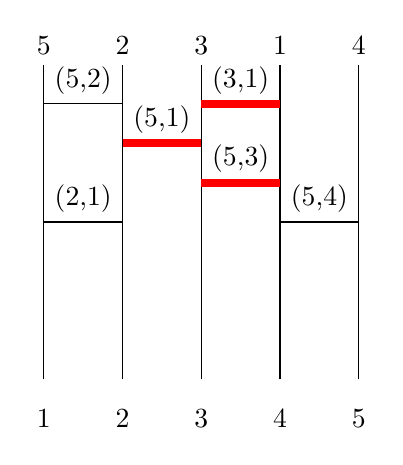
\begin{tikzpicture}
				\draw(0, 0) to (0, 4) node[above]{5};
				\node at (0, -0.5){1};

				\draw(1, 0) to (1, 4) node[above]{2};
				\node at (1, -0.5){2};


				\draw(2, 0) to (2, 4) node[above]{3};
				\node at (2, -0.5){3};

				\draw(3, 0) to (3, 4) node[above]{1};
				\node at (3, -0.5){4};


				\draw(4, 0) to (4, 4) node[above]{4};
				\node at (4, -0.5){5};

				%%Drawing the bars
				\draw(0, 3.5)to (1, 3.5);
					\draw node at (0.5, 3.8){(5,2)};
				\draw[line width=1mm, red](2, 3.5) to (3, 3.5);
					\draw node at (2.5, 3.8) {(3,1)};
				\draw[line width=1mm, red](2, 2.5) to (3, 2.5);
					\draw node at (2.5, 2.8) {(5,3)};
				\draw(3, 2) to (4, 2);
					\draw node at (3.5, 2.3){(5,4)};
				%%4's route, no bars

				%%3s route
				\draw[line width=1mm, red](1, 3) to (2, 3);
					\draw node at (1.5, 3.3) {(5,1)};
				%%2s route
				\draw(0, 2) to (1, 2);
					\draw node at(0.5, 2.3){(2,1)};
			\end{tikzpicture}
		\end{flushright}
	\end{minipage}t
	\caption{Example of a local swap operation. When a right swap operation is permformed
	on the left ladder, the result is the right ladder. When a left swap operation is permformed
	on the right ladder, the result is the left ladder.}
\end{figure}








%%%section on how ladde lotteries relate to other mathematical objects
Despite the fact that ladder lotteries have only been stuidied in and
of themseleves for ten years, they are closely tied to other mathematical 
phenomena that have been studied for much longer. These mathematical phenomena  
 include \emph{Pseudo Lines} which are an arrangement of 
curves on a plane such that given two curves, they only intersect 
at most once and at each intersection, only two curves intersect.See figure --reference--
for a wiring diagrams of the pseudo line arrangement for the 
permutation, $(5,4,3,2,1)$. The other mathematical phenomena is \emph{adjacent transpositions}
which is a swap of two adjacent elements in a permutation. 
\subsection{Ladders and Adjacent Transpositions}
A ladder lottery is a way of sorting a permutation, yet it can also be thought of as 
a decomposition of a permutation into \emph{adjacent transpositions}. \cite{A1} 
An \emph{adjacent transposition} is simply a swap of two adjacent elements in a 
permutation. For example, given the permutation (1, 3, 4, 2), an adjacent 
transposition could be done on the following pairs of elements: 
(1, 3), (3, 4) or (4, 2). Each would result in a unique permutation. 
Simply put, given any arbitrary starting permutation, $\pi$, keep swapping 
adjacent inversions until the identity permutation is reached.  An optimal 
ladder lottery from $\pi's$ optimal ladder set is a minimal sequence of 
adjacent transpositions such that $\pi$ is sorted into the identity permutation; 
each ladder in the set represents a sequence of adjacent transpositions for 
sorting $\pi$ into the identity permutation. For example, given the permutation 
(4, 3, 2, 1) there exists eight ladders in this permutation's optimal ladder set. 
Two of these ladders are found in \ref{fig:ac}:

\begin{figure}[!htp]
    \label{fig:ac}
	\begin{minipage}{0.4\textwidth}
		\centering
	
		\begin{tikzpicture}
			\draw(0, 0) to (0, 4) node[above]{4};
			\draw(2, 0) to (2, 4) node[above]{3};
			\draw(4, 0) to (4, 4) node[above]{2};
			\draw(6, 0) to (6, 4) node[above]{1};
			
			\draw(0, 3.7) to (2, 3.7);
				\draw node at (1, 3.9) {(4, 3)};
			\draw(2, 3.25) to (4, 3.25);
				\draw node at (3, 3.45){(4, 2)};
			\draw(4, 2.75) to (6, 2.75);
				\draw node at (5, 3.0){(4, 1)};
			
			\draw(0, 2.75) to (2, 2.75);
				\draw node at (1, 3.0){(3, 2)};
			\draw(2, 2.25) to (4, 2.25);
				\draw node at (3, 2.5){(3, 1)};
			
			
			\draw(0, 1.75) to (2, 1.75);
				\draw node at (1, 1.95){(2, 1)};
			
			\draw node at (0, -0.5){1};
			\draw node at (2, -0.5){2};
			\draw node at (4, -0.5){3};
			\draw node at (6, -0.5){4};
			
			%%second ladder%%
			\draw(9, 0) to (9, 4) node[above]{4};
			\draw(11, 0) to (11, 4)node[above]{3};
			\draw(13, 0) to (13, 4)node[above]{2};
			\draw(15, 0) to (15, 4)node[above]{1};
			
			\draw(9, 3.7) to (11, 3.7);
				\draw node at (10, 3.9) {(4, 3)};
			\draw(11, 3.25) to (13, 3.25);
				\draw node at (12, 3.45){(4, 2)};
			\draw(13, 2.75) to (15, 2.75);
				\draw node at (14, 3.0){(4, 1)};
			
			\draw(9, 1.25) to (11, 1.25);
				\draw node at (10, 1.5){(3, 1)};
			\draw(11, 2) to (13, 2);
				\draw node at (12, 2.25){(2, 1)};
			
			\draw(11, 0.65) to (13, 0.65);
				\draw node at (12, 0.85){(3, 2)};
			 
			
			\draw node at (9, -0.5){1};
			\draw node at (11, -0.5){2};
			\draw node at (13, -0.5){3};
			\draw node at (15, -0.5){4};	
		\end{tikzpicture}
	
	\end{minipage}
	

	
		
	\caption{The left ladder is one of eight unique ladders from (4,3,2,1)'s optimal ladder set. The right ladder is another one of eight unique ladders form (4,3,2,1)'s optimal ladder set}
		
\end{figure}

From looking at the above ladders, going from top left to bottom right, the left ladder represents the sequence of adjacent transpositions (4,3), (4,2), (4,1),(3,2),(3,1),(2,1) 
whereas the right ladder represent the sequence of adjacent transpositions 
(4, 3),(4, 2),(4, 1),(2, 1),(3, 1),(3, 2). 
Notice how the length of the sequences are the same,because both lengths are equal 
to the minimal number of swaps to sort (4, 3, 2, 1) 
it is simply the order in which the adjacent transpositions occur in the sequence 
that makes the sequences different from each other. 